\documentclass{beamer}

\usetheme{Madrid}
\usecolortheme{default}

\title{Generating chess puzzles with diffusion}
\author{Aatu Selkee et al.}
\institute{Aalto University}
\date{May 8, 2026}


\usepackage[style=verbose, backend=bibtex]{biblatex}
\usepackage{svg}
\usepackage[dvipsnames]{xcolor}

\addbibresource{references.bib}

\begin{document}

\begin{frame}
    \titlepage
\end{frame}


% \section{Introduction}
% \begin{frame}
%     \centering\Huge Introduction
% \end{frame}

\begin{frame}
    \textbf{What is our plan:}
    \begin{itemize}
        \item Follow your paper on chess puzzle generation with the masked diffusion model% \footcite{feng2025generatingcreativechesspuzzles}
        \item Novel contributions
        \begin{itemize}
            \item Condition the generation on the themes and the difficulty of the puzzles
            \item See if predicting the best move helps puzzle generation
            \item Apply RL for the masked diffusion model
            \begin{itemize}
                \item Specifically, we plan to use  ELBO-based Sequence-level Policy Optimization (ESPO)%\footcite{ou2025principledrldiffusionllms}
            \end{itemize}
            \item Open source implementation: \url{https://github.com/naapeli/Generating-open-source-chess-puzzles}
            \item Perhaps make a UI for people to use the model
        \end{itemize}
    \end{itemize}
\end{frame}

\begin{frame}
    \textbf{What is the state of the project:}
    \begin{itemize}
        \item Pretrained three models:
        \begin{itemize}
            \item A model with no conditioning that predicts the puzzle and the solution
            \item A model with conditioning on themes and ratings that predicts the puzzle and the solution
            \item A model with conditioning on themes and ratings that predicts just the puzzle
        \end{itemize}
        \item First good RL results using the model with no conditioning
        \begin{itemize}
            \item ELBO-based Sequence-level Policy Optimization (ESPO) with the replay buffer from your implementation 
        \end{itemize}
        \item Other models have either overfitted and exploded or not improved at all, although, we have not attempted to train them with the latest setup, which worked for the unconditioned model.
    \end{itemize}
\end{frame}

\begin{frame}
    \textbf{What is the state of the project:}
    \begin{itemize}
        \item Challenges:
        \begin{itemize}
            \item Getting both uniqueness and counter-intuitiveness to improve during RL using the models with conditioning.
            \item Improving the best move prediction using RL while maintaining high counter-intuitiveness.
            \item When running SFT for best move prediction, the model forgets puzzle generation capabilities (KL pinning or mixed training could help)
        \end{itemize}
    \item We hope to show that the auxiliary task of best move generation improves puzzle generation.
    \end{itemize}
\end{frame}

% \begin{frame}
%     \textbf{What have we have done so far:}
%     \begin{itemize}
%         \item Pretrained the masked diffusion model to 300 000 steps (validation loss starting to separate from the train loss slightly, but we may try to train a little further)
%         \item Implemented the RL training pipeline
%         \item Implemented the reward functions (as similarly to your implementations as we could based on the paper)
%         \item Early experiments with the RL training
%     \end{itemize}
% \end{frame}

\begin{frame}
    \textbf{Reward function:}
    \begin{itemize}
        \item All metrics are as close as possible to your implementations.
        \item Our reward function does not use principal variation distance to the Lichess dataset nor entropy filtering.
        \item We give a small reward even if a position has a unique solution, but is not counter-intuitive.
        \item Our reward function for the working RL configuration is as follows:
    \end{itemize}
    \begin{equation*}
        R = \begin{cases}
            -2 & if \quad\neg\mathbb{I}_{\text{legal}} \\
            0.1 & if \quad\mathbb{I}_{\text{legal}} \cdot \mathbb{I}_{\text{diversity}} \cdot \mathbb{I}_{\text{unique}} \cdot \neg\mathbb{I}_{\text{counter-intuitive}}\\
            1 & if \quad\mathbb{I}_{\text{legal}} \cdot \mathbb{I}_{\text{diversity}} \cdot \mathbb{I}_{\text{unique}} \cdot \mathbb{I}_{\text{counter-intuitive}}\\
            0 & \quad \text{otherwise}
        \end{cases}
    \end{equation*}
    where $\mathbb{I}_{\text{diversity}} = \mathbb{I}_{\text{intra}, \text{fen}} \cdot \mathbb{I}_{\text{intra}, \text{pv}} \cdot \mathbb{I}_{\text{inter}, \text{fen}} \cdot \mathbb{I}_{\text{piece counts}}$.
\end{frame}

% \begin{frame}
%     \textbf{ESPO:}
%     \begin{itemize}
%         \item Mostly the same as GRPO, but with the ELBO instead of the probability of model generation.
%         \item Optimize the following:
%     \end{itemize}
%     \begin{align*}
%         \mathcal{J}_{\text{seq}}(\pi_\theta) &= \mathbb{E}_{x\sim\mathcal{D},y^{(1:G)}\sim \pi_{\text{old}}(\cdot | x)}\left[ L_i(\theta) \right], \\
%         L_i(\theta) &= \frac{1}{G}\sum_{i=1}^{G} \min(\rho_\text{seq}^{(i)}\hat{A}^{(i)}, \text{clip}(\rho_\text{seq}^{(i)}, 1 - \epsilon, 1 + \epsilon)\hat{A}^{(i)}),
%     \end{align*}
%     where $\rho_{\text{seq}}^{(i)} = \exp(\frac{1}{L}(\mathcal{L}_\theta(y^{(i)} | x) - \mathcal{L}_{\theta_{\text{old}}}(y^{(i)} | x)))$ and $\mathcal{L}$ is the evidence lower bound.

%     \begin{itemize}
%         \item Initial tests with an easy reward have worked well
%         \item If the larger runs do not end up working, we may go back to a more traditional policy gradient.
%     \end{itemize}
% \end{frame}

\begin{frame}
    \begin{figure}
        \begin{columns}
            \begin{column}{0.5\textwidth}
                \centering
                
\includegraphics[width=0.8\textwidth]{figures/reward.pdf} \\
                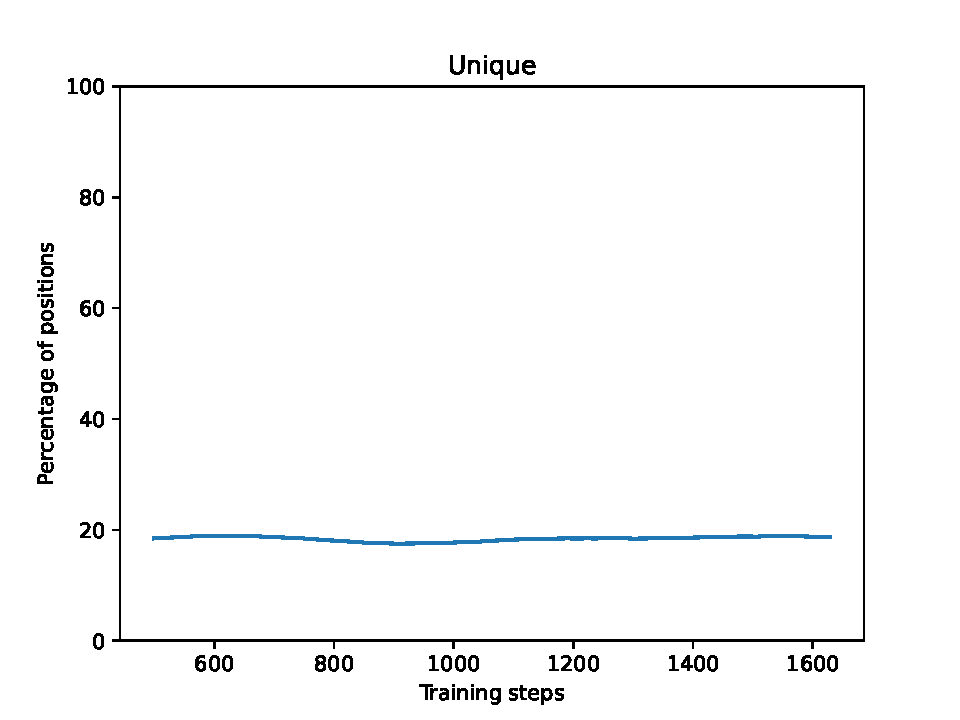
\includegraphics[width=0.8\textwidth]{figures/unique01.pdf}
            \end{column}
            \begin{column}{0.5\textwidth}
                \centering
                
\includegraphics[width=0.8\textwidth]{figures/unique_and_counter_intuitive.pdf} \\
                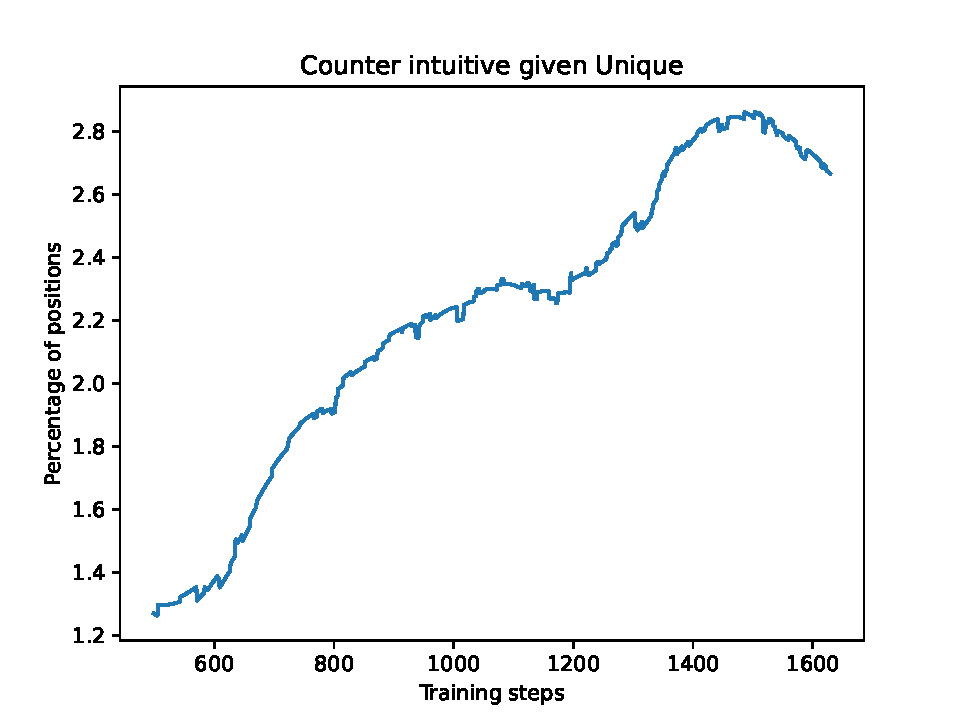
\includegraphics[width=0.8\textwidth]{figures/counter_intuitive_given_unique.pdf}
            \end{column}
        \end{columns}
        \caption{\footnotesize The amount of positions that pass the uniqueness and counter-intuitiveness criteria increases as more gradient updates are made. They improve mainly through improving the counter-intuitiveness of the positions.}
    \end{figure}
\end{frame}

\begin{frame}
    \begin{figure}
        \begin{columns}
            \begin{column}{0.5\textwidth}
                \centering
                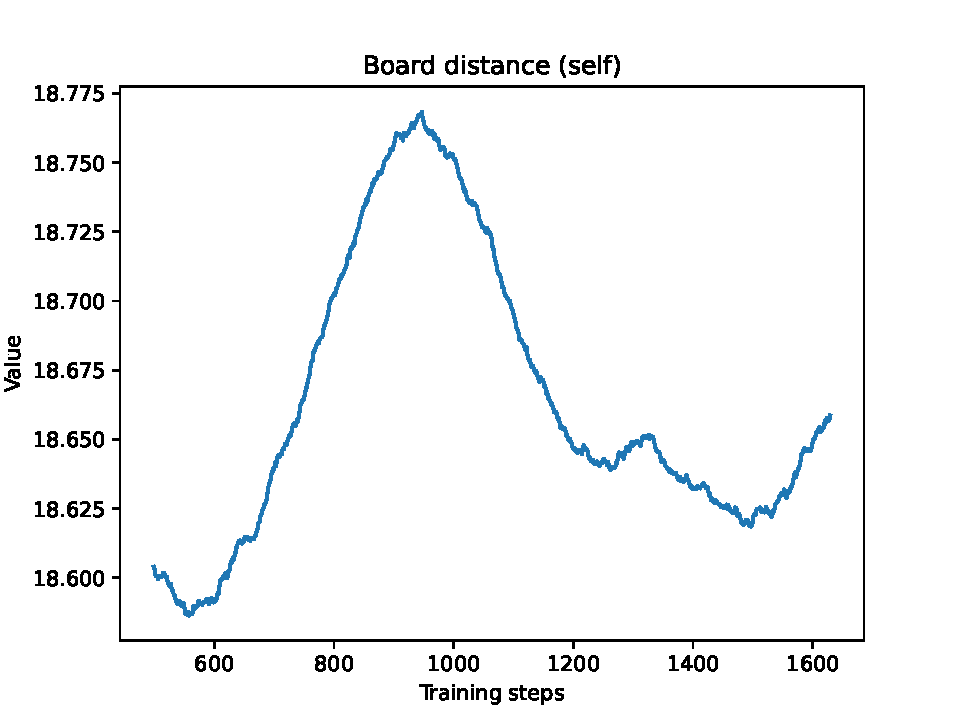
\includegraphics[width=0.8\textwidth]{figures/intra_fen.pdf} \\
                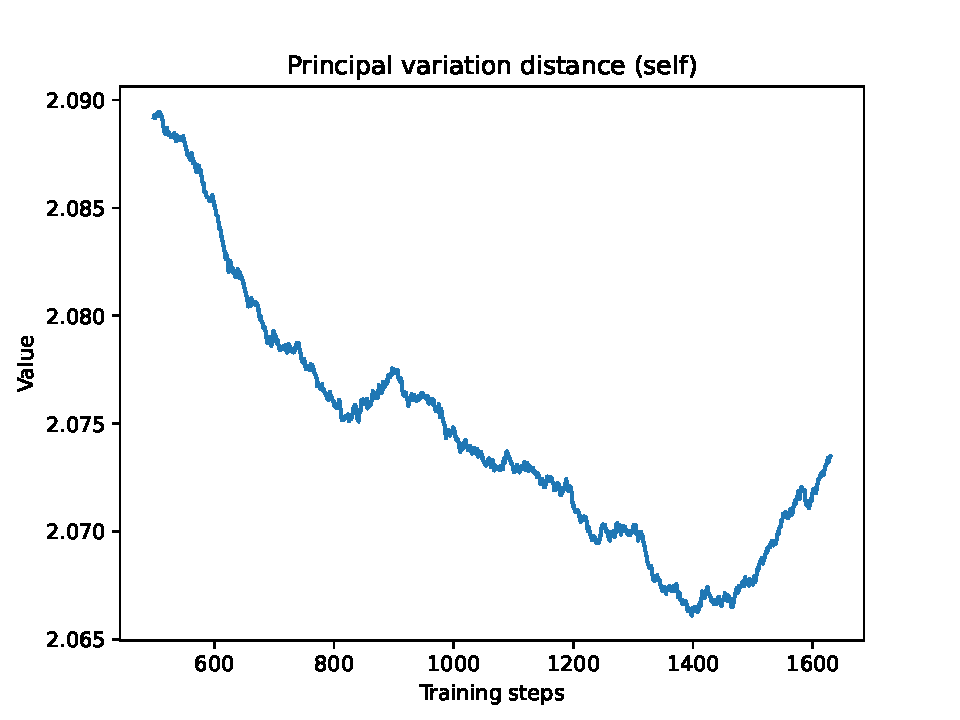
\includegraphics[width=0.8\textwidth]{figures/intra_pv.pdf}
            \end{column}
            \begin{column}{0.5\textwidth}
                \centering
                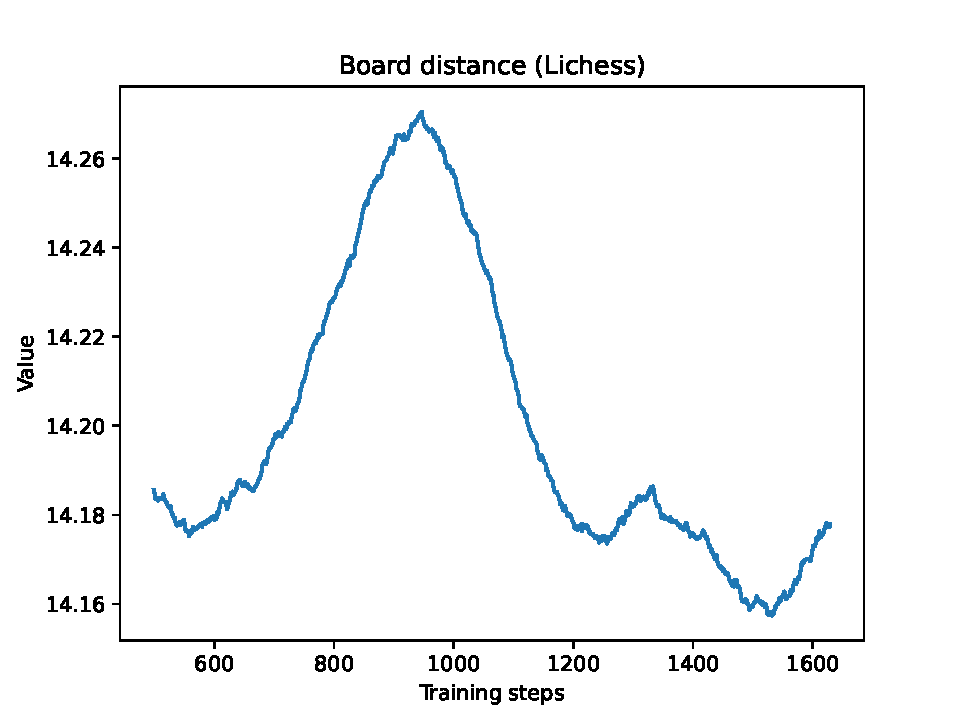
\includegraphics[width=0.8\textwidth]{figures/inter_fen.pdf} \\
                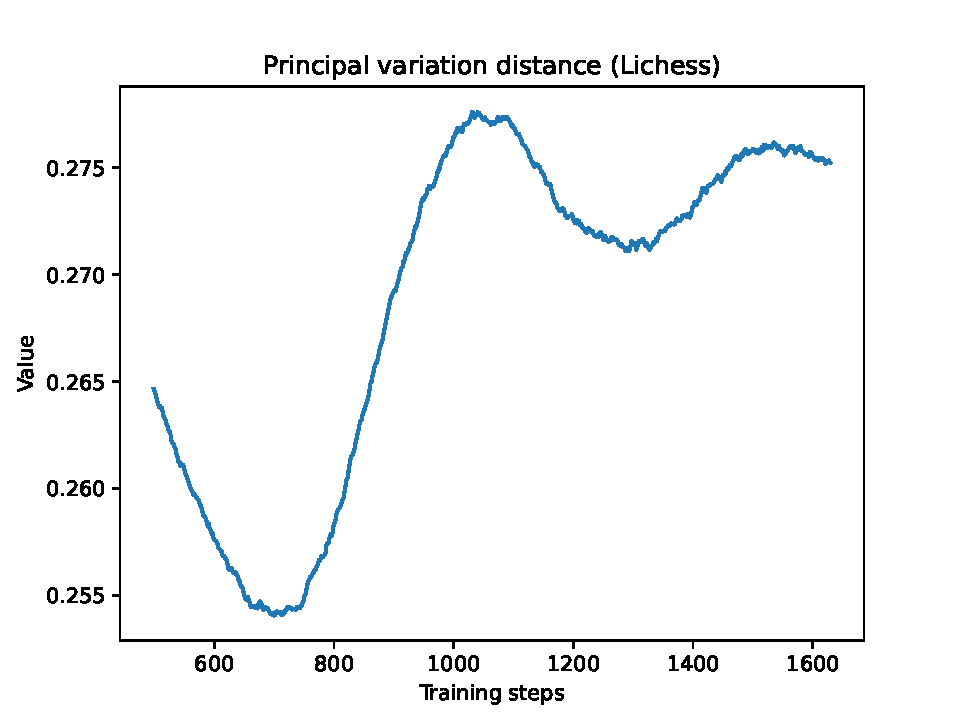
\includegraphics[width=0.8\textwidth]{figures/inter_pv.pdf}
            \end{column}
        \end{columns}
        \caption{\footnotesize The diversity of the positions is high in the beginning and does not meaningfully change during the training. The PV distance to the Lichess dataset increases throughout the training, which is interesting, as it is not a part of our reward function.}
    \end{figure}
\end{frame}

\begin{frame}
    \begin{figure}
        \begin{columns}
            \begin{column}{0.5\textwidth}
                \centering
                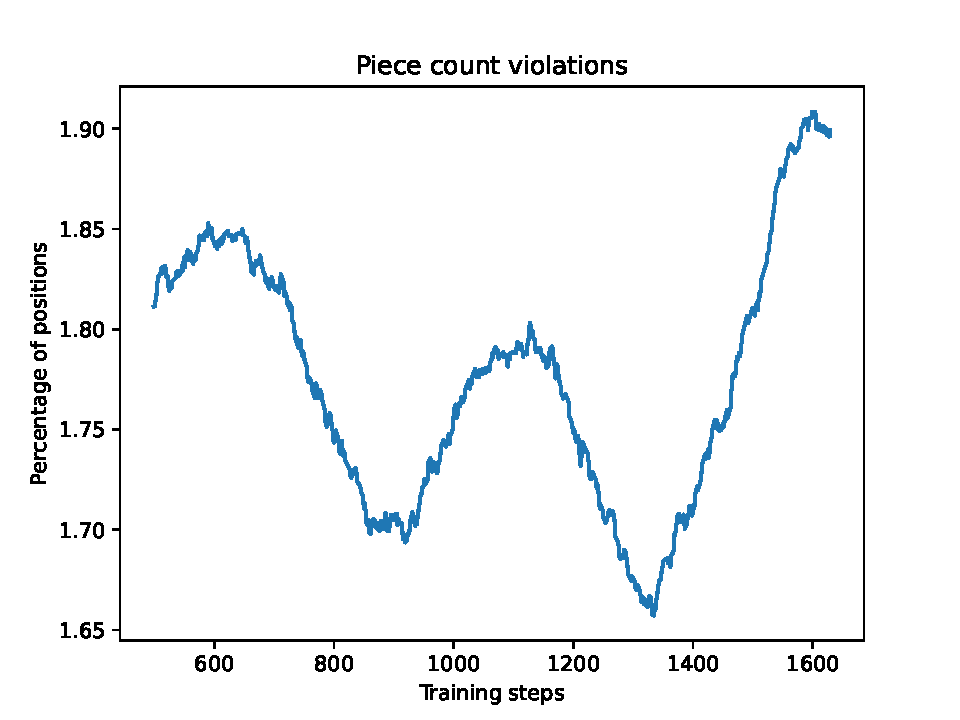
\includegraphics[width=0.8\textwidth]{figures/piece_counts.pdf} \\
                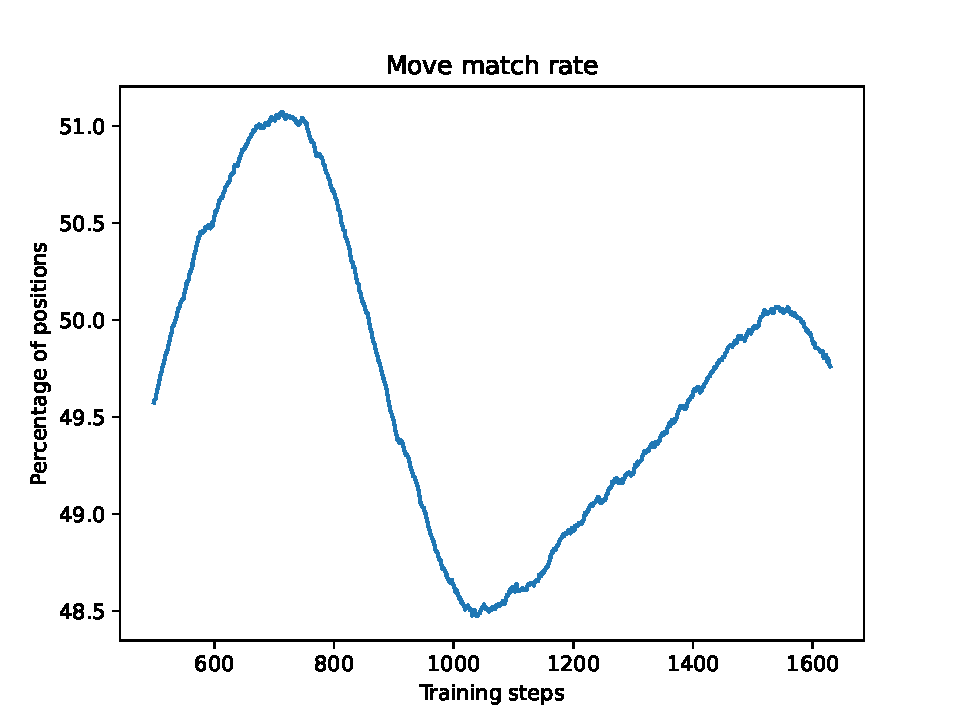
\includegraphics[width=0.8\textwidth]{figures/move_match.pdf}
            \end{column}
            \begin{column}{0.5\textwidth}
                \centering
                
\includegraphics[width=0.8\textwidth]{figures/entropy.pdf} \\
                
\includegraphics[width=0.8\textwidth]{figures/kl_divergence.pdf}
            \end{column}
        \end{columns}
    \caption{\footnotesize The other metrics do not meaningfully change during the training.}
    \end{figure}
\end{frame}

\begin{frame}
    \begin{figure}
        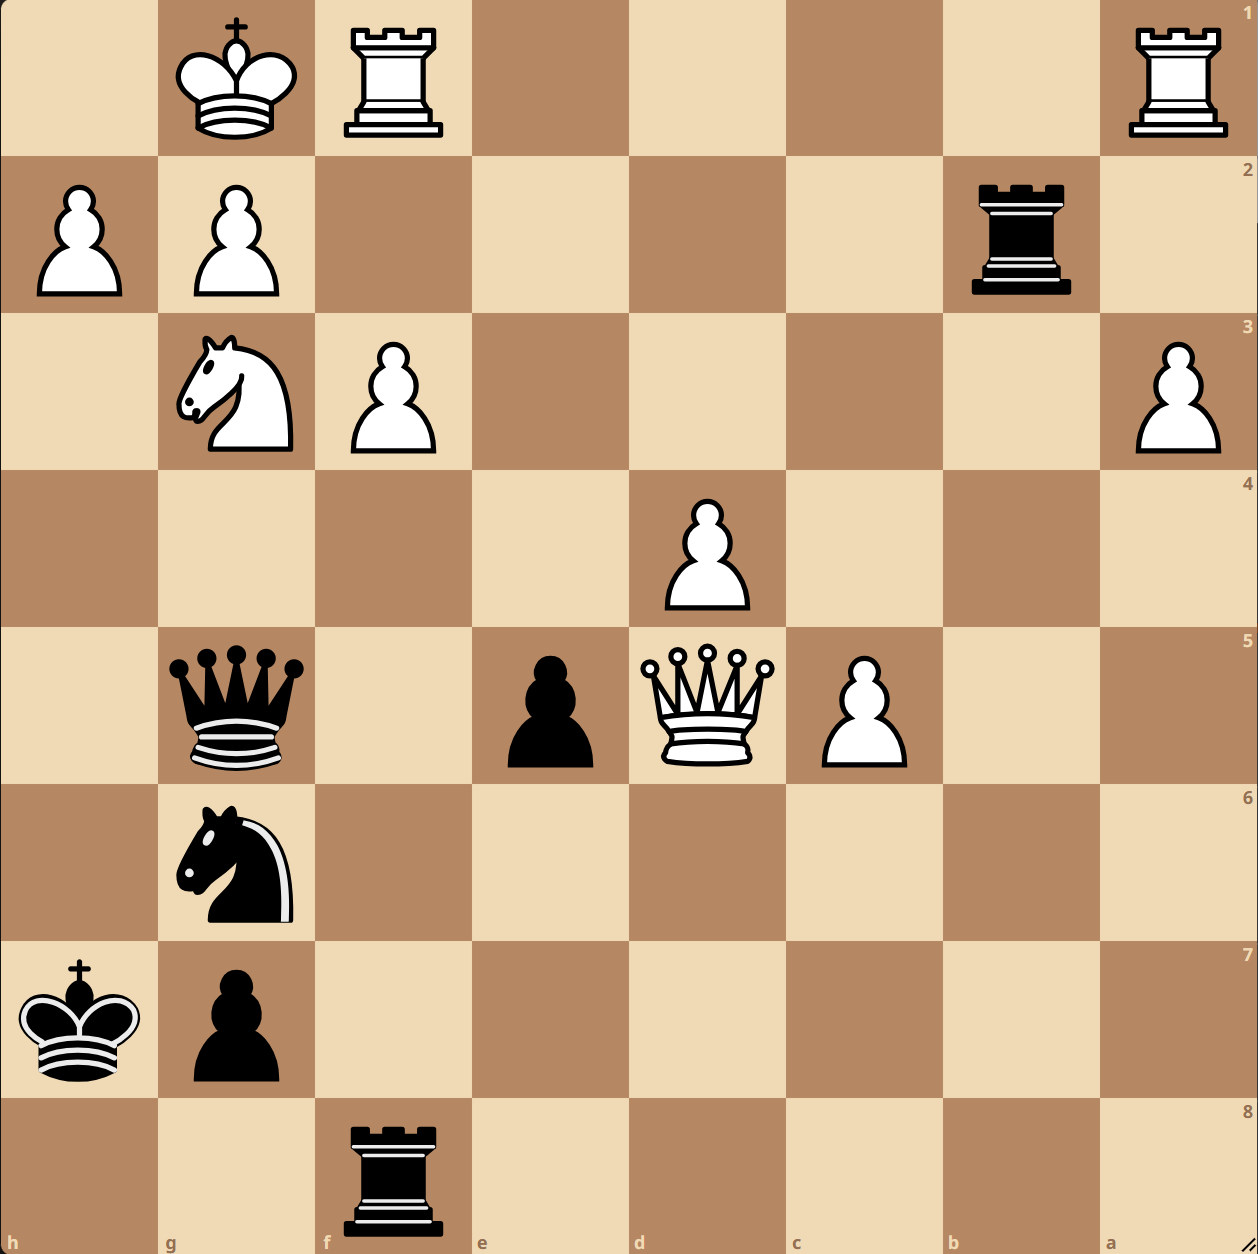
\includegraphics[width=0.65\textwidth]{figures/pos1.png}
        \caption{5r2/6pk/6n1/2PQp1q1/3P4/P4PN1/1r4PP/R4RK1 b - - 0 28}
    \end{figure}
\end{frame}

% \begin{frame}
%     \begin{figure}
%         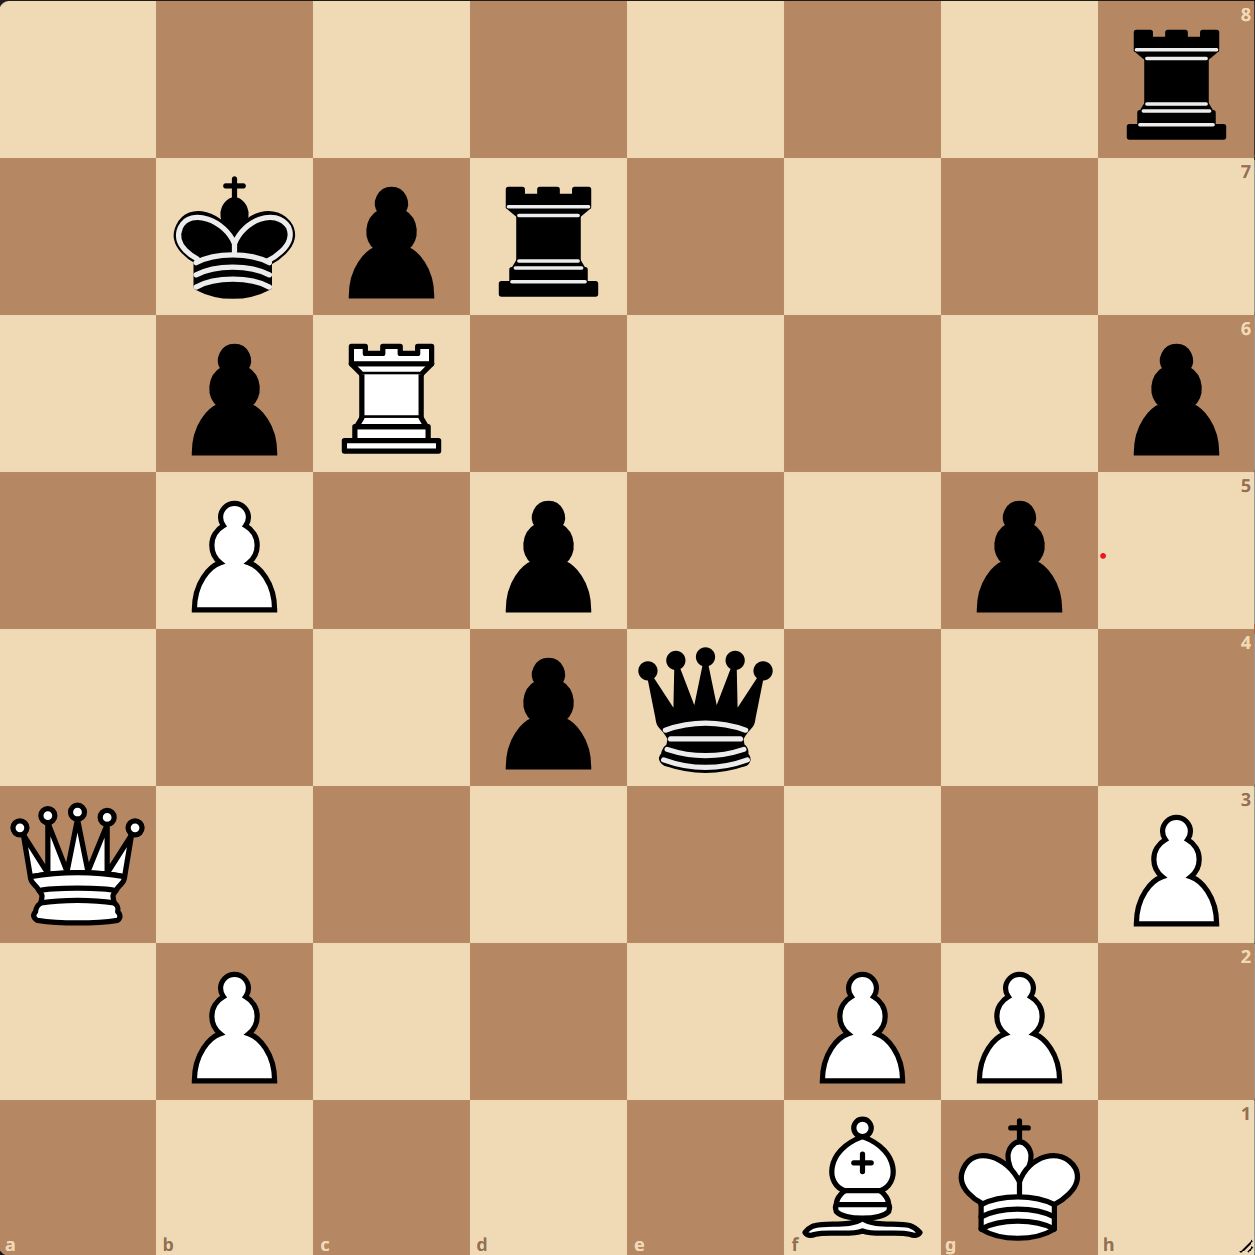
\includegraphics[width=0.65\textwidth]{figures/pos2}
%         \caption{7r/1kpr4/1pR4p/1P1p2p1/3pq3/Q6P/1P3PP1/5BK1 w - - 0 33}
%     \end{figure}
% \end{frame}

\begin{frame}
    \textbf{Questions:}
    \begin{itemize}
        \item We found that the PV distance to the Lichess distribution in our experiments is a lot smaller than in your paper. Do we understand your paper correctly that you sample 2000 positions from the replay buffer and compute the minimum PV distance to those positions?
        \item We tried incorporating the entropy into the loss (via gradient descent) and the reward and found in both cases the model would eventually start generating illegal positions. Did you find anything similar?
        \item What smoothing did you use in the plots of your paper?
        \item Do you have any additional suggestions for research directions we could try?
    \end{itemize}
\end{frame}

\end{document}
